\documentclass{scrartcl}
\usepackage[T1]{fontenc}
\usepackage[utf8]{inputenc}
\usepackage[ngerman]{babel}
\usepackage{amsmath,amssymb}
\usepackage{graphicx}
\usepackage{enumerate}
\usepackage{calc}
\usepackage{ifthen}
\usepackage{multirow}
\usepackage[left=1.5cm, right=1.5cm, top=2.0cm]{geometry}

\newcommand{\replicate}[2]{\ifnum#1>0 #2
	\expandafter\replicate\expandafter{\number\numexpr#1-1}{#2}\fi}

\newcommand{\modulo}[2]{#1-((#1+#2)/#2-1)*#2}

\newcounter{station}\setcounter{station}{1}
\newcounter{ctrA}
\newcounter{ctrB}
\newcounter{currentRow}

\newcounter{noOfStations}\setcounter{noOfStations}{11}

\renewcommand{\arraystretch}{1.5}

%Parameter: {Stationsname}{Messgröße}{miteinander? (0=nein, 1=ja)}
\newenvironment{stationsheet}[3]
{\begin{center} \textbf{\huge Station \arabic{station}: #1}\\[2em]\end{center}
\textbf{\Large Ergebnisse:}\\[1em]
\setcounter{ctrA}{\value{station}}
\setcounter{ctrB}{\value{station}}
\setcounter{currentRow}{1}
\begin{tabular}{|c|c|p{3cm}|p{11cm}|}
\hline
\textbf{Rd.} & \textbf{Nr.} & \textbf{#2} & \textbf{Platz für Strichliste, Bemerkungen, ...}\\ \hline
\replicate{\value{noOfStations}}
{
\multirow{2}{*}{\arabic{currentRow}} & A\arabic{ctrA} & &
\ifthenelse{#3=0}{\\ \cline{2-4}}{\\ \cline{2-2}}
 & B\arabic{ctrB} & & \stepcounter{currentRow}
\setcounter{ctrA}{1+\modulo{\value{ctrA}-2}{\value{noOfStations}}}
\setcounter{ctrB}{1+\modulo{\value{ctrB}}{\value{noOfStations}}}
\\ \hline
}
\end{tabular}
\clearpage
\begin{center}\textbf{\huge Station \arabic{station}: #1}\end{center}
\textbf{\Large Regeln:}\\[1em]
}
{
\textbf{\Large Spielplan:}\\[1em]
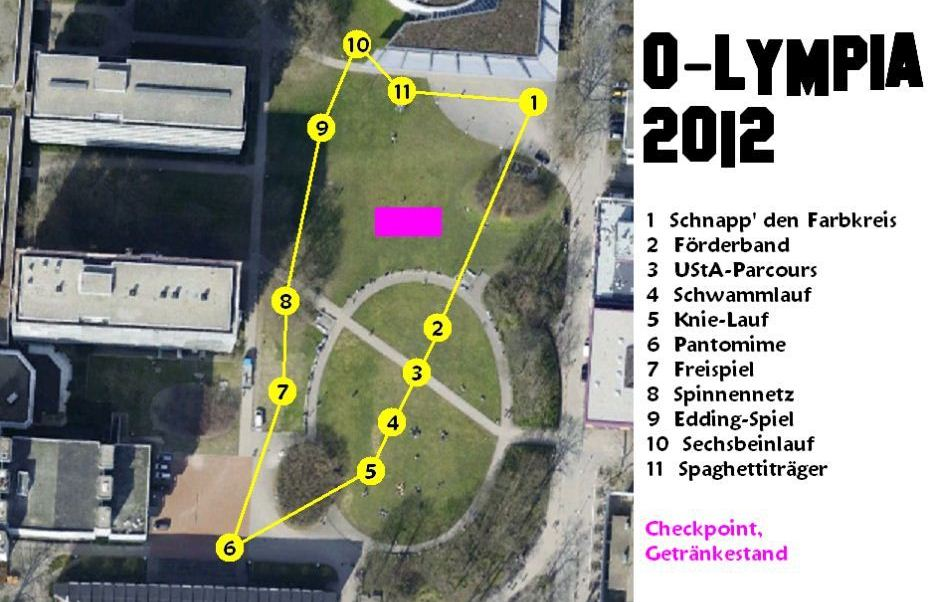
\includegraphics[scale=0.57]{spielplan_11.png}
\addtocounter{station}{1}
\clearpage
}

\pagestyle{empty}

\begin{document}
\shorthandoff{"}
%Regeln Version 13:49, 2. Okt 2012 (Wiki)
\begin{stationsheet}{Schnapp' den Farbkreis}{Anzahl}{0}
Bei diesem Spiel geht es darum, auf einem Tisch befestigte Farbkreise zu "schnappen", immer wenn in einem vorgelesenen Text das entsprechende Farbwort vorkommt.
\begin{itemize}
\item Der Text mit den vielen Farbwörtern ist in drei etwa gleich lange Abschnitte eingeteilt. In jeder Runde treten je zwei Spieler aus der einen gegen zwei Spieler der anderen Gruppe an, wobei sich die in den jeweiligen Runden verwendeten Spielermengen nicht schneiden dürfen, d.h. für dieses Spiel braucht man genau 6 Spieler aus jeder Gruppe. \item Die beiden Spieler aus einer Gruppe sitzen jeweils auf einer Bank an dem Tisch. Außerdem ist vor jedem Spieler eine ca. 3cm breite Markierung für die Position der Hände an der Tischkante angebracht.
\item Nun liest ein Fachschafter einen Text vor, in dem viele Farbwörter vorkommen. Liest er ein Farbwort vor, zu dem ein entsprechender Farbkreis auf dem Tisch liegt, dürfen die Spieler nach dem entsprechenden Farbkreis "schnappen". Schnappen bedeutet, dass man den Farbkreis mit seiner Hand berührt. Es wird notiert, wie oft jede Gruppe am schnellsten "zuschnappt". Es ist irrelevant, ob das Farbwort im Sinne des Textverständnisses tatsächlich ein Farbwort darstellt oder nicht.
\item Alle Spieler dürfen nach allen Farbkreisen schnappen.
\item Alle Spieler müssen für die Dauer des Spiels Schmuck an Händen und Unterarmen (wie z.B. Ringe oder Armbanduhren) ablegen. (Vermeidung von unnötigen Verletzungen)
\item Die Hände der Spieler müssen auf der Markierung bleiben. Näher ran darf man erst nach Nennung des Farbwortes. Hält sich ein Spieler nicht an diese Regel, erhält seine Gruppe eine Negativwertung in Bezug auf die Anzahl der geschnappten Farbkreise. Genauso verhält es sich, wenn ein Spieler einen Farbkreis schnappt, ohne dass die entsprechende Farbe genannt wurde.
\item Ausschlaggebend ist die Anzahl der geschnappten Farbkreise nach der oben beschriebenen Wertung.
\end{itemize}
\end{stationsheet}

\begin{stationsheet}{Förderband}{Paare}{1}
Bei diesem Spiel geht es darum, einen Spieler über eine Art Endlos-Förderband, bestehend aus den anderen Spielern, zu transportieren.
\begin{itemize}
\item Für dieses Spiel muss jede Gruppe 14 Mitspieler stellen. Diese bilden das Förderband. Zusätzlich wird ein leichter Spieler benötigt, der auf dem Förderband transportiert wird.
\item Die beiden 14er-Gruppen bilden zwei Spielerketten, die sich gegenüberstehen und die Hände ausstrecken. Der leichte Spieler wird von zwei Stationsbetreuern auf das Förderband gehoben.
\item Nun bewegen die Förderband-Spieler den leichten Spieler Stück für Stück über das Förderband. Durch den Transport des leichten Spielers werden am Anfang des Förderbandes nach und nach Spielerpaare frei. Diese reihen sich am Ende des Förderbands wieder ein.
\item Es ist darauf zu achten, dass niemand herunterfällt (das ist der eigentliche Sinn des Spiels). Sollte dies doch geschehen oder wird der verfügbare Platz überschritten, wird das Spiel vom Startpunkt fortgesetzt, d.h. alle Spieler müssen ihre Anfangsposition einnehmen. Der Zähler für die freigewordenen Spielerpaare bleibt dabei bestehen.
\item Ausschlaggebend ist die Anzahl der während der Spielzeit freigewordenen Spielerpaare.
\end{itemize}
\end{stationsheet}

\begin{stationsheet}{UStA-Parcours}{Ergebnis}{0}
Regeln stellt der UStA auf.\\[1em]
\end{stationsheet}

\begin{stationsheet}{Schwammlauf}{Wassermenge}{0}
Bei diesem Spiel geht es darum, mithilfe eines Schwamms eine möglichst große Wassermenge über eine gegebene Distanz zu transportieren. Die Gruppen spielen dabei parallel.
\begin{itemize}
\item Jeder Gruppe stehen ein Schwamm und zwei Stöcke zur Verfügung. Mithilfe von Wasser in einer Wanne am Startpunkt bringt man möglichst viel Wasser in dem Schwamm unter. Dann transportieren zwei Spieler den Schwamm mithilfe der Stöcke zum Zielpunkt. Der Schwamm darf mit keinem Körperteil, also nur mit den Stöcken berührt werden! Am Zielpunkt angekommen, darf der Schwamm in die Hand genommen und über einem Eimer ausgewrungen werden. Die Spieler kehren mit dem Schwamm zurück zum Startpunkt. Auf dem Rückweg darf man diesen mit der Hand transportieren.
\item Der eben beschriebene Vorgang wiederholt sich laufend, bis die Spielzeit abgelaufen ist.
\item Fällt der Schwamm auf dem Transportweg hinunter, muss er mithilfe der Stöcke wieder aufgehoben werden.
\item Wird der Schwamm auf dem Transportweg mit der Hand berührt, gilt dieser Transport als ungültig und es muss vom Startpunkt neu begonnen werden.
\item Nach Beendigung des Spiels wird gemessen, wie viel Wasser sich im Eimer der jeweiligen Gruppe befindet. Ausschlaggebend ist die gemessene Wassermenge.
\end{itemize}
\end{stationsheet}

\begin{stationsheet}{Knie-Lauf}{Wassermenge}{0}
Bei diesem Spiel geht es darum, eine mit Wasser gefüllte Getränkeflasche zwischen den Knien über eine gewisse Distanz zu transportieren und dort in einen Eimer zu entleeren, ohne diese mit den Händen zu berühren. Die Gruppen spielen dabei parallel.
\begin{itemize}
\item Am Startpunkt wird eine Getränkeflasche mit Wasser gefüllt, die einer der Spieler dann zwischen seine Knie klemmt. Der Spieler muss nun mitsamt der Flasche zu seinem Eimer gelangen und das Wasser dort ausschütten. Hierbei darf die Flasche nicht anders als zwischen den Knien klemmend berührt werden, auch nicht zum Ausschütten! Geschieht dies doch, muss vom Startpunkt neu begonnen werden. Sollte obendrein noch nicht-gültiges Wasser in den Eimer gelangen, so ist dies von den Stationsbetreuern auf dem Ergebnisbogen zu vermerken!
\item Es ist nicht gestattet, dass der gerade laufende Spieler von anderen Spielern aktiv unterstützt wird. (Zum Eimer getragen werden, wie letztes Jahr oft geschehen, ist nicht mehr gestattet.)
\item Das Ausschütten des Wassers gelingt leicht, wenn sich der Spieler mit der Flasche in einer liegestütze-ähnlichen Position über den Eimer beugt. Dies ist vor Spielbeginn allen mitzuteilen.
\item Ausschlaggebend ist die nach Ablauf der Spielzeit gemessene Wassermenge in jedem Eimer.
\end{itemize}
\end{stationsheet}

\begin{stationsheet}{Pantomime}{Begriffe}{1}
Bei diesem Spiel geht es darum, dass zwei Spieler (je einer aus beiden Gruppen) von allen anderen Spielern pantomimisch dargestellte Begriffe erraten. Die Gruppen spielen dabei miteinander.
\begin{itemize}
\item Die beiden Begriffe-Rater und der Stationsbetreuer, welcher die Begriffe anzeigt, stehen allen Darstellern gegenüber, sodass diese die Begriffe und die beiden Begriffe-Rater die Darstellungen sehen können. Hierbei steht der Stationsbetreuer etwas weiter hinten als die Begriffe-Rater, welche sich nicht umdrehen dürfen. Damit die Darsteller die Begriffe sehen können, stellen sich die Begriffe-Rater nicht direkt vor den Stationsbetreuer, sondern etwas seitlich.
\item Die Reihenfolge der Begriffe wurde im Vorfeld der O-Lympia festgelegt. Jedoch ist es bei jedem Begriff durch die Darsteller oder Rater möglich, diesen durch Ansage von "weiter" zu überspringen. Eine Wiederholung der übersprungenen Begriffe ist nicht möglich!
\item Während dem Spiel dürfen die Darsteller nicht sprechen. Kommt dies doch vor, so ist der gerade darzustellende Begriff zu überspringen.
\item Das Spiel endet, wenn alle Begriffe erraten oder übersprungen worden sind oder die Spielzeit abgelaufen ist. Ausschlaggebend ist die Anzahl erratener Begriffe.
\end{itemize}
\end{stationsheet}

\begin{stationsheet}{Freispiel}{Punkte}{0}
Bei diesem Spiel geht es darum, 10 Punkte (nichtnegativ, ganzzahlig) an zwei Gruppen zu verteilen, wobei die Gruppen weitestgehend selbst entscheiden dürfen, wie dies vonstatten geht. Die Gruppen spielen dabei gegeneinander.\begin{itemize}
\item Vor Beginn der Spielzeit dürfen die Spieler innerhalb der Gruppen bereits besprechen, wie sie die Punkte gerne aufteilen würden. Eine Verhandlung mit der gegnerischen Gruppe ist erst nach Ankündigung des Spielbeginns erlaubt.
\item Während der Spielzeit müssen die Gruppen zunächst miteinander verhandeln, wie sie die 10 Punkte zwischen sich aufteilen möchten. Hierbei ist es vollkommen gleichgültig, wie die Punkte verteilt werden, solange beide Gruppen (und die Stationsbetreuer) mit der Art der Punkteaufteilung einverstanden sind. Anschließend treten sie das ausgehandelte Spiel an.
\item Nach Ablauf der Spielzeit werden die bis dahin aufgeteilten Punkte vergeben. Haben die Gruppen sich darauf geeinigt, in mehreren Runden Teile der Punkte zu sammeln, und sind noch nicht alle Runden gespielt, so sind nur die bis dahin gesammelten Punkte zu vergeben; der Rest verfällt. Kommt es zu keiner Einigung bezüglich der Punkte-Aufteilung, bekommt niemand Punkte.
\end{itemize}
\end{stationsheet}

\begin{stationsheet}{Spinnennetz}{Passagen}{1}
Bei diesem Spiel geht es darum, Spieler durch ein durch zwischen zwei Bäumen aufgespanntes Seil entstandenes Netz zu transportieren. Die Gruppen spielen dabei miteinander.
\begin{itemize}
\item Alle Spieler beider Gruppen befinden sich zunächst auf einer Seite des Spinnennetzes. Nun müssen die Spieler nacheinander durch Passieren der 15 Löcher im Netz auf die andere Seite gelangen. Häufig braucht man hierbei die Mithilfe von anderen Spielern (z.B. zum Durchhieven bei höher gelegenen Löchern).
\item Jedes der Löcher darf maximal zweimal benutzt werden. Ein Stationsbetreuer achtet darauf, dass diese Regel eingehalten wird und weist die Spieler ggf. darauf hin, dass sie das Loch nicht mehr benutzen sollen. Das Spiel endet, wenn alle Löcher zweimal passiert wurden oder die Spielzeit abgelaufen ist.
\item Die Stationsbetreuer zählen mit, wie viele Spieler das Netz ohne Berührungen passieren. Wird das Netz zwar berührt, aber nur sehr geringfügig, so darf man dies als halbe Passage zählen.
\item Alle Spieler, die das Netz bereits passiert haben, halten sich hinter dem Netz auf und diejenigen, die es noch nicht passiert haben, vor ihm. Insbesondere darf jeder Spieler das Netz nur einmal passieren.
\item Ausschlaggebend ist die Anzahl der gemeisterten Passagen innerhalb der Spielzeit.
\end{itemize}
\end{stationsheet}

\begin{stationsheet}{Edding-Spiel}{Weite}{0}
Bei diesem Spiel geht es eigentlich darum, einen Edding möglichst weit von einer geradlinigen Markierung aufzustellen. Da das Spiel auf dem Rasen stattfindet, werden statt der Eddings Flaschen verwendet. Die Gruppen spielen dabei parallel.
\begin{itemize}
\item Beide Gruppen erhalten je eine Flasche als Spielobjekt. Diese können sie unter Einbeziehung aller Spieler ihrer Gruppe an beliebiger Stelle hinter der Markierung aufstellen. Es sind beliebig viele Versuche erlaubt, solange die Spielzeit läuft. Nach jedem gelungenen Versuch wird die Distanz zwischen Markierung und Flasche gemessen.
\item Es sind keinerlei Hilfsmittel erlaubt. Die Aufstellung der Flasche darf nur mithilfe der körperlichen Kräfte der Spieler erfolgen.
\item Keiner der Spieler darf während des Aufstellungsvorgangs den Boden hinter der Markierung mit irgendeinem Körperteil oder Kleidungsstück berühren. Der Aufstellungsvorgang gilt als beendet, wenn alle Spieler wieder sicher vor der Markierung stehen.
\item Ausschlaggebend ist die größte gemessene Distanz jeder Gruppe.
\end{itemize}
\end{stationsheet}

\begin{stationsheet}{Sechsbeinlauf}{Durchgänge}{0}
Bei diesem Spiel geht es darum, dass aneinandergebundene Fünf-Personen-Teams eine Strecke ablaufen. Die Gruppen spielen dabei parallel.
\begin{itemize}
\item Es stellen sich fünf Personen nebeneinander auf und werden mithilfe von O-Phasen-T-Shirt-Fetzen an den Füßen aneinandergebunden, sodass nur der linke Fuß des (von vorne betrachtet) am weitesten rechts stehenden Spielers bzw. der rechte Fuß des am weitesten links stehenden Spielers frei sind. Das so gebildete sechsbeinige Konstrukt läuft nun eine gewisse Distanz ab, die durch eine Markierung versehen ist, läuft um die Markierung herum und wieder zurück.
\item Während ein Sechsbein unterwegs ist, darf sich das folgende Sechsbein bereit machen (sprich, seine Halbfüße miteinander verbinden).
\item Es gibt genügend Platz für alle. Daher ist es nicht gestattet, ein gegnerisches Sechsbein bei seinem Lauf zu stören, auf welche Art auch immer. Sollte dies doch vorkommen, ist der Durchgang der störenden Gruppe als ungültig zu werten.
\item Ausschlaggebend ist die Anzahl der vollständig absolvierten Durchgänge innerhalb der Spielzeit.
\end{itemize}
\end{stationsheet}

\begin{stationsheet}{Spaghettiträger}{Durchgänge}{1}
Ziel des Spiel ist es, eine Dose mittels einer Spaghetti, die an jedem Ende von einem Spieler in den Mund genommen wird, zu transportieren. Die Gruppen spielen dabei miteinander.
\begin{itemize}
\item Je ein Spieler der einen und ein Spieler der anderen Gruppe erhalten zusammen eine Spaghetti, die sie durch die Lasche der Dose schieben. Nun nehmen beide Spieler je ein Ende der Spaghetti in den Mund und die beiden können so die Dose transportieren. Nach Anheben der Dose absolvieren die beiden Spieler eine Distanz bis hinter eine Markierung und kehren wieder zurück. Dort müssen sie die Dose wieder abstellen. Sobald die Dose sicher steht, können sie die Spaghetti loslassen und mit den Händen herausziehen. Anschließend dürfen die nächsten beiden Spieler antreten usw.
\item Wenn eine Spaghetti unterwegs bricht, führt dies zu einer erheblichen Erschwernis, aber nicht zum Zwangsabbruch des Durchgangs. Fällt hingegen die Dose zu Boden, so ist der Durchgang ungültig. Genauso ist der Durchgang ungültig, wenn die Dose beim Absetzen am Zielpunkt umfällt, nachdem die Spieler die Spaghetti losgelassen haben. Ebenfalls ungültig sind Versuche, die nicht mit der vollständigen Spaghetti durchgeführt werden. Am Ende des Versuchs muss die gesamte Spaghetti rekonstruierbar sein, d.h. es ist nicht erlaubt, die Spaghetti während des Durchgangs durch Aufessen zu kürzen.
\item Tritt einer der Spieler auf eine (heruntergefallene) Dose und ist diese dadurch so kaputt, dass man sie nicht mehr hinstellen kann, so bekommen die Gruppen eine dreifache Negativwertung in Bezug auf die gültigen Durchgänge.
\item Wird während eines Durchgangs die Dose mit einem Körperteil oder die Spaghetti anders als mit dem Mund berührt, ist der entsprechende Durchgang ungültig. Ein Durchgang beginnt durch Anheben der Dose und endet, wenn diese wieder sicher auf dem Tisch steht.
\item Ausschlaggebend ist die Anzahl der vollständig absolvierten Durchgänge während der Spielzeit.
\item Tipps (bitte an die Spieler weitergeben): Spaghetti beim Dosentransport unter Spannung halten, dann brechen sie nicht so häufig. Beim Abstellen der Dose so in die Hocke gehen, dass man nicht mit den Köpfen aufeinander zugeht.
\end{itemize}
\end{stationsheet}
\end{document}